\documentclass{article}

\usepackage{graphicx}
\usepackage{amsmath}
\usepackage{caption}
\usepackage{subcaption}
\usepackage{listings}
\usepackage[hidelinks]{hyperref}
\usepackage{enumitem}
\usepackage{geometry}
\usepackage{biblatex}

\renewcommand{\contentsname}{Table of Contents}
\addbibresource{sad.bib}
\geometry{
 a4paper,
 left=20mm,
 right=20mm,
 top=20mm,
 bottom=25mm,
 }

\begin{document}

\begin{titlepage}
\begin{center}
\vspace*{1cm}

\Huge
\textbf{Project 01: Home Safe}

\vspace{0.5cm}
\Large
\textit{Software Architecture Design} \\
\textit{SAD Version 1}

\vspace{1cm}

\textbf{Team 01}

\vspace{0.5cm}

\text{Marina Seheon (Manager)} \\
\text{Andrei Phelps (Document Manager)} \\
\text{Luke McDougall (Lead Software Engineer)} \\
\text{Jack Vanlyssel} \\
\text{Spoorthi Menta} \\
\text{Vamsi Krishna Singara} \\

\vspace{1cm}

\begin{figure}[h]
    \centering
    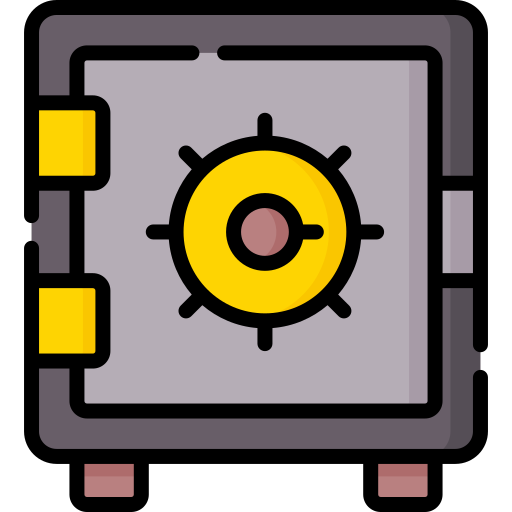
\includegraphics[width=0.25\textwidth]{docs/figs/safe.png}
    \caption*{Image courtesy of Flaticon.com \cite{flaticonSafeDeposit}.}
    \label{fig:safeIcon}
\end{figure}

\vspace{7cm}

\Large
\textbf{CS460: Software Engineering} \\

\end{center}
\end{titlepage}

\newpage

\tableofcontents

\newpage

\section{Introduction}
This document presents the architectural framework for the HomeSafe software solution. Grounded in the Software Requirements Specification (SRS), this documentation provides a thorough breakdown of the core requirements defining the HomeSafe ecosystem. For those keen on exploring the intricate facets of HomeSafe’s functionalities, interfacing elements, and logical flow, the SRS serves as a reservoir of in-depth knowledge. The design principles laid out here are meticulously aligned with the directives established in the SRS. \\ \\
In addition to an overarching outline of the system's layout, enthusiasts will discover in-depth explanations of individual design elements, accompanied by illustrative samples and potential design limitations. For an organized reading experience, key terminologies, pivotal to the document's context, are clarified in Section 2. Sections 3 and 4 respectively peel back the layers on the software's architectural nuances and the intricate details of its components. Meanwhile, Section 5 enriches readers with real-world scenarios, highlighting practical applications and use cases.

\section{Definition of Terms}
This section provides definitions for critical terms recurrently utilized throughout the document. This section can be a reference point for readers engaging with the content.

\begin{enumerate}
    \item[I.] \textbf{Auxiliary}: An additional or secondary power source that supports the main or primary power supply. An auxiliary power source is typically used to provide backup, redundancy, or temporary power when the main power source is unavailable, disrupted, or insufficient.
    \item[II.] \textbf{Bio-Metric Scanner}: A technology that identifies and authenticates users based on their unique biological characteristics, typically fingerprints, retina patterns, or other traits.
    \item[III.] \textbf{Central Processing Unit (CPU)}: Also known as a central processor or a main processor, it serves as the core component of any computer. This unit carries out the essential functions of executing program instructions, including tasks like calculations, logical operations, control functions, and managing input/output processes.
    \item[IV.] \textbf{Microcontroller}: A microcontroller is a small integrated circuit serving as the central processing unit (CPU) of a safe's electronic system. It contains a processor, memory, and input/output ports and can include programmable capabilities. Microcontrollers manage the safe's tasks, user input, security protocols, and control functions, including locks, interface interactions, and external device communication.
    \item[V.] \textbf{Personal Identification Number (PIN)}: A numerical code that serves as a security credential used to authenticate and verify the identity of an individual. PINs are commonly used in various systems, such as electronic devices, bank accounts, and access control systems, to ensure that only authorized users can gain access.
    \item[VI.] \textbf{Two-Factor Authentication (2FA)}: A security protocol that requires users to provide two distinct forms of verification to access a system. This commonly involves a combination of something known (such as a password) and something possessed (such as a generated code or biometric information), adding an extra layer of security and protection against unauthorized access \cite{identityautomationTwoFactorAuthentication}.
\end{enumerate}

\section{Architecture Design Overview}
This section delves deeply into the intricate software architecture underpinning the HomeSafe lock system. As we navigate through, emphasis will be placed on understanding the individual software components, their respective roles, and the intricate web of interactions among them. To provide a holistic view, a comprehensive diagram will be showcased, illustrating the dynamic interplay and control flow that exists between these software modules. Following the visual representation, there will be a discussion on each module's specific functionalities, their significance in the overall system, and the synergies they create when working together. By the end of this section, readers will gain a comprehensive insight into the software backbone that powers the HomeSafe lock system.

\begin{figure}[h]
    \centering
    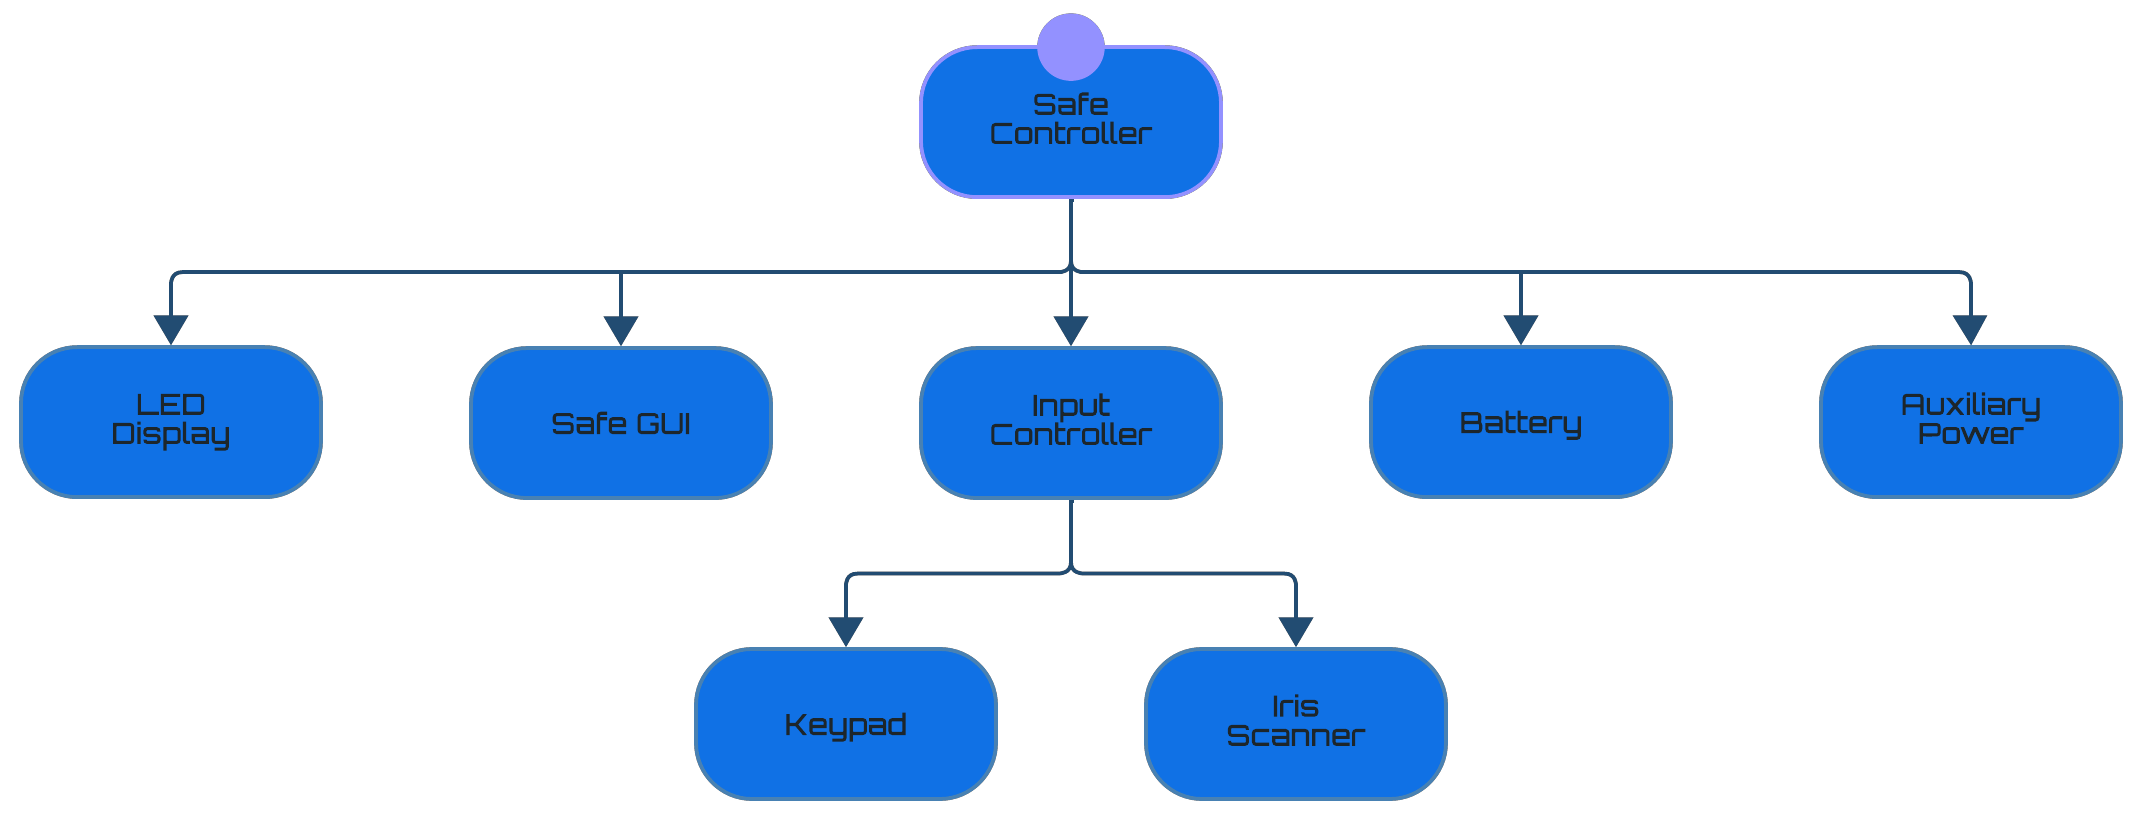
\includegraphics[scale=0.32]{docs/figs/architecture_design.png}
    \caption{Architecture Design Diagram \cite{lucidLucidVisual}}
    \label{fig:diagram1}
\end{figure}

\subsection{Design Description}
This section delves into the core software components: SafeController(), IrisScanner(), and Keypad() classes, and their interactions. \\ \\
The SafeController() acts as the central command, promptly initializing the InputController(), Screen(), AuxPower(), and SafeGUI() components. When a user presents their eye to the biometric module, the IrisScanner() class springs into action, recognizing the eye pattern and sending the data to the InputController(). This data is then passed to the SafeController() for validation against stored iris patterns. \\ \\
Concurrently, the Keypad class oversees the user interactions with the keypad. When a user keys in a 6-digit PIN, the InputController() processes this input and coordinates with the SafeController() for verification, similar to the iris scanning procedure. \\ \\
After consolidating the authentication details, the SafeController() manages the overarching system dynamics. Depending on the verification outcomes, the SafeController() triggers reactions in the Screen(), Battery(), and the tactile feedback mechanisms. These software components seamlessly bridge with their tangible equivalents: the display unit, power units, and the tactile feedback system of the keypad().

\section{Component Specifications}
This section delves into the intricacies of the software components illustrated in the design diagram outlined in Figure \ref{fig:diagram1}. It offers a comprehensive perspective on each software component and underscores their interdependencies.

\subsection{Microcontroller (Software)}
The \texttt{SafeController} class acts as the microcontroller in the software architecture. It manages the state of the safe and coordinates between different components such as the screen, Keypad, and SafeGUI. It holds a list of users and maintains the current user and state.

\begin{itemize}
    \item \texttt{setState(SafeState newState)}: This method is used to change the state of the safe. It handles states like waiting for an iris scan, setting iris, initial PIN setup, normal, closed, adding a new user, locked, and master verification.
    \item \texttt{handleMasterVerification()}: This method is invoked when the state is set to master verification. It displays a message to enter the master PIN.
    \item \texttt{handleWaitingForIris()}: and \texttt{handleSettingIris()}: These methods are used to handle the states related to the iris scanner. They display messages to guide the user in iris scanning.
    \item \texttt{handleInitialPinSetup()}: and \texttt{handleNormalState()}: These methods handle the initial PIN setup and normal states by displaying appropriate messages.
    \item \texttt{handleUnlockedState()}: This method handles the unlocked state by displaying a message and opening the safe GUI after a delay.
    \item \texttt{checkPIN(String enteredPIN)}: This method checks the entered PIN against the stored PINs for various states and displays appropriate messages.
    \item \texttt{checkIris(String irisName)}: This method checks the entered iris name against the stored iris names and handles the state accordingly.
    \item \texttt{setIrisForCurrentUser(String irisName)}: This method sets the iris name for the current user.
\end{itemize}
\textbf{Dependencies}:
\begin{itemize}
    \item Depends on the \texttt{Screen} class to display messages.
    \item Depends on the \texttt{SafeGUI} class to handle the GUI-related tasks.
    \item Depends on the \texttt{User} class to manage user information.
    \item Depends on the \texttt{SafeState} enum to manage the state of the safe.
\end{itemize}

\subsection{Input Controller (Software)}
The \texttt{InputController} class handles the input from the user via the IRIS scanner and Keypad. It manages the power state and interacts with the \texttt{Screen}, \texttt{SafeController}, and \texttt{PINManager} to handle various inputs.

\begin{itemize}
    \item \texttt{handleKeyInput(String key)}: This method handles the key inputs from the user. If the power is on, it appends the key entry to the screen. Otherwise, it does nothing.
    \item \texttt{handleCancel()}: This method handles the cancel operation by removing the last key entry from the screen.
    \item \texttt{handleEnterButton()}: This method is invoked when the enter button is pressed. It checks the PIN entered by calling the \texttt{checkPIN} method of the \texttt{SafeController} and clears the key entry from the screen.
    \item \texttt{handlePowerButton()}: This method handles the power button press. It toggles the power state and sets the state of the \texttt{SafeController} accordingly.
\end{itemize}
\textbf{Dependencies}:
\begin{itemize}
    \item Depends on the \texttt{Screen} class to display and manage key entries.
    \item Depends on the \texttt{SafeController} class to check the PIN and set the state of the safe.
    \item Depends on the \texttt{PINManager} class for managing PIN-related operations.
\end{itemize}

\subsection{GUI Manager (SafeGUI, Software)}
The \texttt{SafeGUI} class is responsible for managing the graphical user interface of the safe. It handles the display of images representing the safe's state (open, closed), the keypad for PIN entry, and buttons for various controls.

\begin{itemize}
    \item \texttt{start(Stage primaryStage)}: This method initializes the primary stage of the application, setting up the images, button panel, screen, and keypad. It also handles mouse clicks on the image view to transition to a close-up view of the safe.
    \item \texttt{openSafe()}: This method changes the image to show the safe in an open state and hides the screen component, keypad, and button box. It also provides a button to close the safe.
    \item \texttt{closeSafe()}: This method is used to close the safe. It changes the state of the \texttt{safeController} to closed, updates the image to show the safe in a closed state, and makes the screen component, keypad, and button box visible again.
\end{itemize}
\textbf{Dependencies}:
\begin{itemize}
    \item Depends on the \texttt{Screen} class to manage the display screen of the safe.
    \item Depends on the \texttt{KeyPad} class for handling keypad-related operations.
    \item Depends on the \texttt{ButtonPanel} class for managing the button panel.
    \item Depends on the \texttt{SafeController} class to manage the state of the safe.
    \item Depends on the \texttt{SafeState} enum to manage the state of the safe.
\end{itemize}
This class is crucial for providing a user-friendly interface, allowing users to interact with the safe effectively and efficiently, and ensuring that the state of the safe is visually represented to the user at all times.

\subsection{Iris Scanner (Software)}
The Iris Scanner functionality is embedded within the \texttt{SafeController} class. It is responsible for handling the iris scanning and verification process to ensure secure access to the safe.

\begin{itemize}
    \item \texttt{handleWaitingForIris()}: This method displays a message on the screen indicating that the system is waiting for an iris scan.
    \item \texttt{handleSettingIris()}: This method prompts the user to scan their iris for setting or updating the iris data in the system.
    \item \texttt{checkIris(String irisName)}: This method checks the scanned iris data against the stored iris data for the current user. If the iris data matches, it transitions the state to unlocked; otherwise, it displays an error message and reverts to the normal state.
    \item \texttt{setIrisForCurrentUser(String irisName)}: This method sets the iris data for the current user in the system.
\end{itemize}
\textbf{Dependencies}:
\begin{itemize}
    \item Depends on the \texttt{Screen} class to display messages related to the iris scanning process.
    \item Depends on the \texttt{User} class to manage and verify user data, including iris data.
    \item Interacts with various states defined in the \texttt{SafeState} enum to manage the iris scanning and verification process flow.
\end{itemize}
This component ensures that only authorized users whose iris data matches the stored data can access the safe, providing an additional layer of security beyond the PIN authentication.

\subsection{Battery (Software)}

The \texttt{Battery} class in the software represents the hardware component responsible for powering the safe and its associated features. It is crucial for ensuring the continuous and reliable operation of the safe, providing the necessary power for the microcontroller, screen, and other components to function effectively.

\begin{itemize}
    \item \texttt{startBatteryDepletion()}: This method begins the battery depletion process, continuously checking the battery level and issuing warnings or stopping the safe operations as necessary.
    \item \texttt{discharge(double amount)}: This method discharges the battery by a specified amount.
    \item \texttt{isVoltageSafe(int voltage)}: This method checks if the charging voltage is within a safe range.
    \item \texttt{charge(int amount, int voltage)}: This method charges the battery by a specified amount, ensuring the voltage is safe.
    \item \texttt{isLow()}: This method checks if the battery is low based on the predefined low battery threshold.
    \item \texttt{getChargeLevel()}: This method returns the battery's current charge level.
    \item \texttt{getRemainingWorkingTime()}: This method returns the remaining working time of the battery in minutes.
\end{itemize}
\textbf{Dependencies}: \\ \\
The \texttt{Battery} class does not depend on other classes but is crucial for the operation of the \texttt{SafeController}, \texttt{Screen}, and other components that require power to function.

\section{Sample Use Cases}
This section offers two use cases showcasing varied scenarios involving HomeSafe. Each example elucidates the user's actions sequentially. Furthermore, with every user action, the reactions from the related system components are detailed.

\subsection{Initial Setup}
In this scenario, the user has just acquired their new HomeSafe and wishes to initialize and configure their access credentials before turning off the safe for subsequent use.

\begin{enumerate}
    \item User removes the HomeSafe from the packaging and places the safe in their desired location.
    \item User removes manual containing the Master PIN from the packaging.
    \item The User presses the power button on the keypad to power the system on.
    \begin{enumerate}
        \item[$\bullet$] Battery power from the primary power source activates the safe components.
        \item[$\bullet$] Microcontroller is activated and awaiting input.
        \item[$\bullet$] Keypad is activated and awaiting input.
        \item[$\bullet$] LED Display prompts the user to enter a 6-digit Master PIN.
    \end{enumerate}
    \item User enters 6-digit Master PIN and presses ENTER.
    \begin{enumerate}
        \item[$\bullet$] Authentication Manager verifies Master PIN.
        \item[$\bullet$] LED Display prompts the user to enter a new 6-digit PIN.
        \item[$\bullet$] The Keypad awaits further input from the user.
    \end{enumerate}
    \item User inputs a 6-digit PIN they wish to use, and presses ENTER.
    \begin{enumerate}
        \item[$\bullet$] LED Display prompts the user to re-enter the 6-digit PIN.
        \item[$\bullet$] The Keypad awaits further input from the user.
    \end{enumerate}
    \item User positions their eye before Iris Scanner until they hear a "BEEP."
    \begin{enumerate}
        \item[$\bullet$] LED Display prompts the user to verify Iris Scan (repeat the previous process).
        \item[$\bullet$] Iris Scanner awaits further input from the user.
    \end{enumerate}
    \item User presses the POWER button on the keypad to power down HomeSafe.
    \begin{enumerate}
        \item[$\bullet$] Power provided by the primary power supply is halted.
        \item[$\bullet$] The Microcontroller and all other safe components are no longer active.
    \end{enumerate}
\end{enumerate}

\subsection{Authorization}
In this scenario, the user has previously configured their Iris Scan and PIN and now seeks to access the safe utilizing those credentials.

\begin{enumerate}
    \item The User presses the power button on the keypad to power the system on.
    \begin{enumerate}
        \item[$\bullet$] Battery power from the primary power source activates the safe components.
        \item[$\bullet$] Microcontroller is activated and awaiting input.
        \item[$\bullet$] Keypad is activated and awaiting input.
        \item[$\bullet$] LED Display prompts the user to enter a 6-digit Master PIN.
    \end{enumerate}
    \item User enters their PIN and presses ENTER.
    \begin{enumerate}
        \item[$\bullet$] Authentication Manager verifies PIN.
        \item[$\bullet$] LED Display prompts the user to provide an Iris Scan.
        \item[$\bullet$] Iris Scanner becomes active and waits for user input.
    \end{enumerate}
    \item User positions their eye before Iris Scanner until they hear a "BEEP."
    \begin{enumerate}
        \item[$\bullet$] Authentication Manager verifies Iris Scan.
        \item[$\bullet$] LED Displays "Authentication Successful" to the user.
        \item[$\bullet$] Locking Mechanism status is changed to UNLOCKED.
    \end{enumerate}
    \item User opens the safe.
    \begin{enumerate}
        \item[$\bullet$] InputController is disabled.
        \item[$\bullet$] LED Displays "Door Open" to the user.
        \item[$\bullet$] Timer starts. An alarm starts if the door is open for more than 120 seconds.
    \end{enumerate}
    \item User closes the safe.
    \begin{enumerate}
        \item[$\bullet$] InputController is re-enabled.
        \item[$\bullet$] LED Displays "Door Closed" to the user.
        \item[$\bullet$] Timer starts. The safe powers itself down if the door is closed for more than 120 seconds without user input on the keypad.
    \end{enumerate}
    \item User presses the POWER button on the keypad to power down HomeSafe.
    \begin{enumerate}
        \item[$\bullet$] Power provided by the primary power supply is halted.
        \item[$\bullet$] The Microcontroller and all other safe components are no longer active.
    \end{enumerate}

\end{enumerate}

\newpage

\printbibliography

{\parindent0pt}

\end{document}
